\documentclass{beamer}
\usetheme[pageofpages=de,% String used between the current page and the
                         % total page count.
          bullet=circle,% Use circles instead of squares for bullets.
          titleline=true,% Show a line below the frame title.
          alternativetitlepage=true,% Use the fancy title page.
          titlepagelogo=../img/fse_ministerio_ancho_texto.png%,% Logo for the first page.
	  %watermark=junta_girado,
          %watermarkheight=75px,% Height of the watermark.
          %watermarkheightmult=4,% The watermark image is 4 times bigger
                                % than watermarkheight.
          ]{Torino}

\usepackage[spanish]{babel} % Para separar correctamente las palabras
\usepackage[utf8]{inputenc} % Este paquete permite poner acentos y eñes usando codificación utf-8

\usepackage{color}

\author{IES Gonzalo Nazareno\\
IES Los Albares\\
IES La Campiña\\
IES Ingeniero de la Cierva\\
\vspace{.5cm}

\includegraphics[width=0.2\textwidth]{cc_by_sa.png}}
\title{IaaS en educación}
\institute{Proyecto de Innovación\\ {\color{white} .\\} \emph{Implantación y
    puesta a punto de la infraestructura de un cloud computing privado para el
    despliegue de servicios en la nube}}  

\begin{document}
\setlength{\parskip}{.2cm}

\begin{frame}[t,plain]
\titlepage
\end{frame}

\begin{frame}
  \frametitle{Cloud Computing}
\end{frame}

\begin{frame}
  \frametitle{Evolución metodológica}
  \begin{itemize}
  \item A la par de la evolución tecnológica, se ha producido una evolución en
    los métodos de enseñanza, que podríamos separar en 3 fases:
    \begin{itemize}
    \item Primera fase: Utilización de equipos físicos
    \item Segunda fase: Utilización de máquinas virtuales
    \item Tercera fase: Utilización de IaaS
    \end{itemize}
  \item Estas fases no son excluyentes: una fase siempre puede incluir las
    anteriores.
  \item Todas tienen ventajas e inconvenientes, pero la tercera fase ofrece
    escenarios imposibles de utilizar anteriormente.

  \end{itemize}
\end{frame}

\begin{frame}
  \frametitle{Evolución metodológica. Primera fase}
  \begin{columns}
    \column{.6\textwidth}
    \begin{itemize}
    \item Utilización de máquinas físicas
      \begin{itemize}
      \item Una máquina por alumno
      \item Algunos servidores compartidos
      \end{itemize}
      \item Pros:
      \begin{itemize}
      \item Fácil despliegue y puesta en marcha
      \end{itemize}
      \item Contras:
      \begin{itemize}
      \item Prácticas muy limitadas por número de equipos y tipo de
        configuraciones
      \item Hardware poco variado
      \item Prácticas muy ``académicas''
      \item Muchos tiempos muertos entre prácticas
      \end{itemize}
    \end{itemize}
    \column{.4\textwidth}
    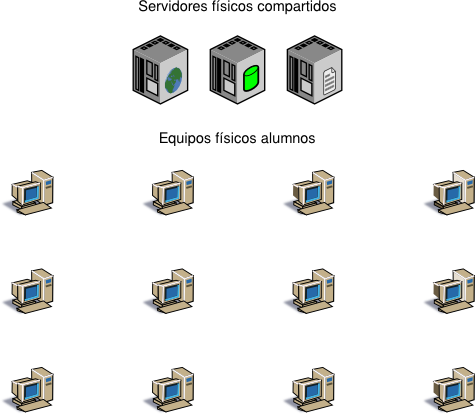
\includegraphics[width=\columnwidth]{../img/epoca1.png}
  \end{columns}
\end{frame}

\begin{frame}
  \frametitle{Evolución metodológica. Segunda fase}
  \begin{columns}
    \column{.6\textwidth}
    \begin{itemize}
    \item Utilización de máquinas virtuales
      \begin{itemize}
      \item Una máquina por alumno
      \item Varias máquinas virtuales por máquina física
      \end{itemize}
      \item Pros:
      \begin{itemize}
      \item Cada alumno dispone de un entorno ``completo'' e independiente
      \item Prácticas menos rígidas
      \item Se aprende virtualización de forma transversal
      \end{itemize}
      \item Contras:
      \begin{itemize}
      \item Entorno más complejo
      \item Requiera equipos actualizados para los alumnos
      \end{itemize}
    \end{itemize}
    \column{.4\textwidth}
    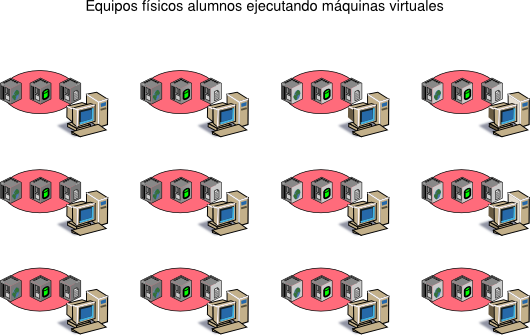
\includegraphics[width=\columnwidth]{../img/epoca2.png}
  \end{columns}
\end{frame}

\begin{frame}
  \frametitle{Evolución metodológica. Tercera fase}
  \begin{columns}
    \column{.6\textwidth}
    \begin{itemize}
    \item Utilización de IaaS
      \begin{itemize}
      \item Un equipo convencional por alumno
      \item IaaS privado de la organización
      \end{itemize}
      \item Pros:
      \begin{itemize}
      \item Enorme variedad de prácticas
      \item Utilización de entornos preconfigurados
      \item Simulación de entornos reales complejos
      \item Equipos básicos para los alumnos
      \item Se aprende IaaS de forma transversal
      \end{itemize}
      \item Contras:
      \begin{itemize}
      \item Sistema muy centralizado
      \item Imprescindible administración del Cloud
      \item Inversión inicial importante
      \end{itemize}
    \end{itemize}
    \column{.4\textwidth}
    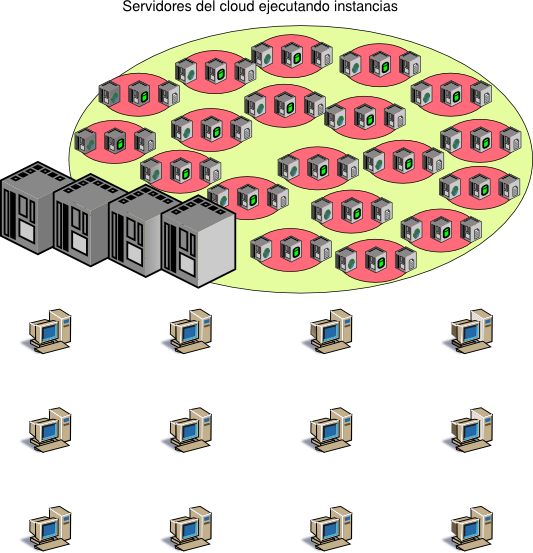
\includegraphics[width=\columnwidth]{../img/epoca3.png}
  \end{columns}
\end{frame}

\begin{frame}
  \frametitle{Simulación de entornos reales}
  Un entorno real es difícil de simular con MVs en un PC por sus
    propias limitaciones, pero en un IaaS es asumible:
    \begin{itemize}
    \item Se puede simular una red con un número importante de equipos
    \item Se puede utilizar la diversidad que se quiera de SOs
    \item Este entorno ``real'' pueden utilizarlo conjuntamente todos los
      alumnos
    \item Puede estar disponible durante todo el curso sin interferir con otras
      asignaturas
    \item Con el tiempo y el uso irán apareciendo conflictos y problemas reales
    \end{itemize}
\end{frame}
\begin{frame}
  \frametitle{Nueva forma de aprendizaje}
  \begin{itemize}
  \item La utilización de IaaS en el ámbito académico conlleva una nueva forma
    de aprender
  \item Con el uso de MVs se había impuesto una forma de aprender que no era
    siempre la mejor, por ejemplo:
    \begin{itemize}
    \item Para utilizar un SGBD había que instalarlo y configurarlo antes
    \item Para desplegar una aplicación web, había que configurar previamente
      todo el servidor de aplicaciones
    \item Para hacer prácticas de ZFS había que instalar Solaris o FreeBSD
    \end{itemize}
    \item Un IaaS puede contar con gran cantidad de imágenes preconfiguradas de
      sistemas con muy diversas configuraciones $\Rightarrow$ La forma de
      aprender no viene condicionada por la necesidad de una configuración
      previa, por ejemplo:
      \begin{itemize}
      \item Primero se utiliza el SGBD durante varias clases.
      \item Posteriormente, cuando sea oportuno, se aprende a instalarlo y
        configurarlo
      \end{itemize}
  \end{itemize}
\end{frame}

\begin{frame}
  \frametitle{Escenarios (I)}
  \begin{description}
  \item[Instalación y configuración de un servicio]
  \end{description}
  Los pasos típicos a seguir serían:
  \begin{itemize}
  \item Cada alumno inicia una instancia del SO en el que va a instalar el
    servicio (no es necesario que previamente sepa instalar ese SO).
  \item Realiza la instalación del servicio
  \item Realiza la configuración del servicio. Si esta configuración dura
    más de una clase, suspende la instancia y la reinicia en la siguiente
    clase.
  \item Una vez terminada la configuración puede crear una instantánea para
    utilizarla como base en posteriores prácticas.
  \item Si algún alumno no ha podido realizar la configuración correctamente
    podrá utilizar la instantánea de un compañero en clases posteriores.
  \end{itemize}
\end{frame}

\begin{frame}
  \frametitle{Escenarios (II)}
  \begin{description}
  \item[Despliegue de una aplicación web]
  \end{description}
  Los pasos típicos a seguir serían:
  \begin{itemize}
  \item Se prepara una imagen de un sistema en el que se configura de forma
    precisa un completo servidor web con todos los módulos necesarios. Se
    instala y configura un servidor git u otro scm.
  \item Cada alumno inicia una instancia de la imagen anterior y transfiere la
    aplicación web desde su equipo.
  \item Comprueba el funcionamiento en un servidor remoto (la instancia) con
    similares características que tendría en un servidor remoto real.
  \item En caso de que tenga que utilizar la instancia durante más de una clase,
    suspende y reinicia cuando sea necesario.
  \item En caso de fallos o errores, puede crear una nueva instancia a partir de
    la imagen inicial o de una instantánea guardada previamente.
  \end{itemize}
\end{frame}

\begin{frame}
  \frametitle{Escenario (III)}
  \begin{description}
  \item[Utilización de herramientas de sistemas]
  \end{description}
  \begin{itemize}
  \item Se prepara una imagen del sistema que se quiera utilizar, por ejemplo
    una imagen de un SO con soporte ZFS.
  \item Cada alumno inicia una instancia de la imagen anterior sin necesidad de
    saber previamente cómo se instala.
  \item Se asocian a la instancia varios volúmenes volátiles.
  \item Se realizan prácticas de ZFS con los volúmenes anteriores.
  \item Cuando se dominen las herramientas se plantea una instalación del SO
    sobre ZFS
  \end{itemize}
\end{frame}

\begin{frame}
  \frametitle{Escenarios. Resumen}
  \begin{itemize}
  \item Esto no son más que tres ejemplos suficientemente diferentes para ver
    las enormes posibilidades que se abren.
  \item En general, pueden plantearse prácticas más complejas, inviables en el
    esquema tradicional de uso de máquinas virtuales por la complejidad de
    configurar el escenario inicial y por los problemas que acarrea una
    equivocación del alumno durante el desarrollo de la práctica.
  \item Además las prácticas no interfieren con otras asignaturas, parar la
    práctica y continuar otro día es tan simple como suspender la instancia y
    reanudarla cuando se precise.
  \end{itemize}
\end{frame}

\begin{frame}
  \frametitle{Aprendizaje transversal}
  \begin{itemize}
  \item El hecho de utilizar IaaS no como fin en sí mismo sino como herramienta
    para aprender otros temas provoca que el alumno se familiarice fácilmente
    con la tecnología.
  \item Este aprendizaje adquirido de forma continua es mucho más significativo
    que si se impartiera como un tema en una asignatura.
  \item En la mayoría de los casos es suficiente con esto, salvo en los
    estudiantes de Administración de Sistemas, que necesariamente tendrán que
    profundizar más en la materia.
  \end{itemize}
\end{frame}

\begin{frame}
  \frametitle{Administración del Cloud}
  
\end{frame}

\begin{frame}
  \frametitle{Inversión inicial}
  \begin{itemize}
  \item Al opta por software libre, la principal inversión son los servidores
    que formarán el cloud de infraestructura.
  \item \textbf{Configuración mínima}: 3 servidores (1 gestión del cloud y 2 para
    ejecución de instancias)
  \item \textbf{Configuración recomendada}: 2 servidores para gestión (en HA), 1
    para almacenamiento y 4 o más para ejecución de instancias
  \item Para la gestión del cloud es suficiente un equipo de características
    mínimas.
  \item Para la ejecución de instancias es necesario procesadores potentes y
    mucha memoria RAM (entre 512 MiB y 2 GiB por instancia) 
  \item El almacenamiento depende del almacenamiento permanente que sea
    necesario.
  \item Sistema fácilmente escalable, se puede empezar por una
    configuración mínima e ir añadiendo componentes año a año.
  \end{itemize}
\end{frame}
\end{document}
